\documentclass[12pt]{article}
\title{\textbf{NATIONAL INSTITUTE OF TECHNOLOGY, RAIPUR(C.G)}}
\usepackage{graphicx}
\graphicspath{{Images/}}


\author{SACHIN KUMAR YADAV\\sachin.1107sk@gmail.com\\Roll No: 21111047}
\date{January 26, 2022}
\begin{document}
\maketitle

\begin{figure}[h]
\centering

\includegraphics[scale=0.8]{nit.jpg}
\caption{National Institute of Technology, Raipur}
\end{figure}

\textbf{ASSIGNMENT-1 OF BASIC BIO-MEDICAL ENGINEERING}\\\\


\section{Nebulizer}
%first paragraph

In medicine, a $nebulizer$ is a machine or a drug delivery device which is used to administer medication in the form of a mist inhaled into the lungs.\\
$Nebulizer$ are commonly used for the treatment of ashthma, cystic fibrosis, and other respiratory diseases or disorders. They use oxygen,compressed air or $ultrasonic power$ power to break up solutions and suspensions into small $aerosol$ droplets that are inhaled from the Mouthpiece of the device. As we have already learnt aerosol  is a mixture of gas and solid or liquid particles.\\
\begin{figure}[h]
\centering
\includegraphics[scale=0.6]{nebu.jpg}
\caption{Nebulizer image}
\end{figure}

%second paragraph
\subsection{Types of nebulizers}
There are three main types of nebulizers available:\\
\textbf{Jet nebulizers} make an aerosol out of medications using a compressed gas (like air). These are the most common type of nebulizers.\\
\textbf{Ultrasonic nebulizers} make an aerosol via high-frequency vibrations. These are more commonly used in hospitals and typically are not for personal use.\\
\textbf{Mesh nebulizers} use a mesh cap with tiny holes that help dispense medication in a very efficient way. These nebulizers are newer and often more effective than jet nebulizers\\
\begin{figure}[h]
\centering
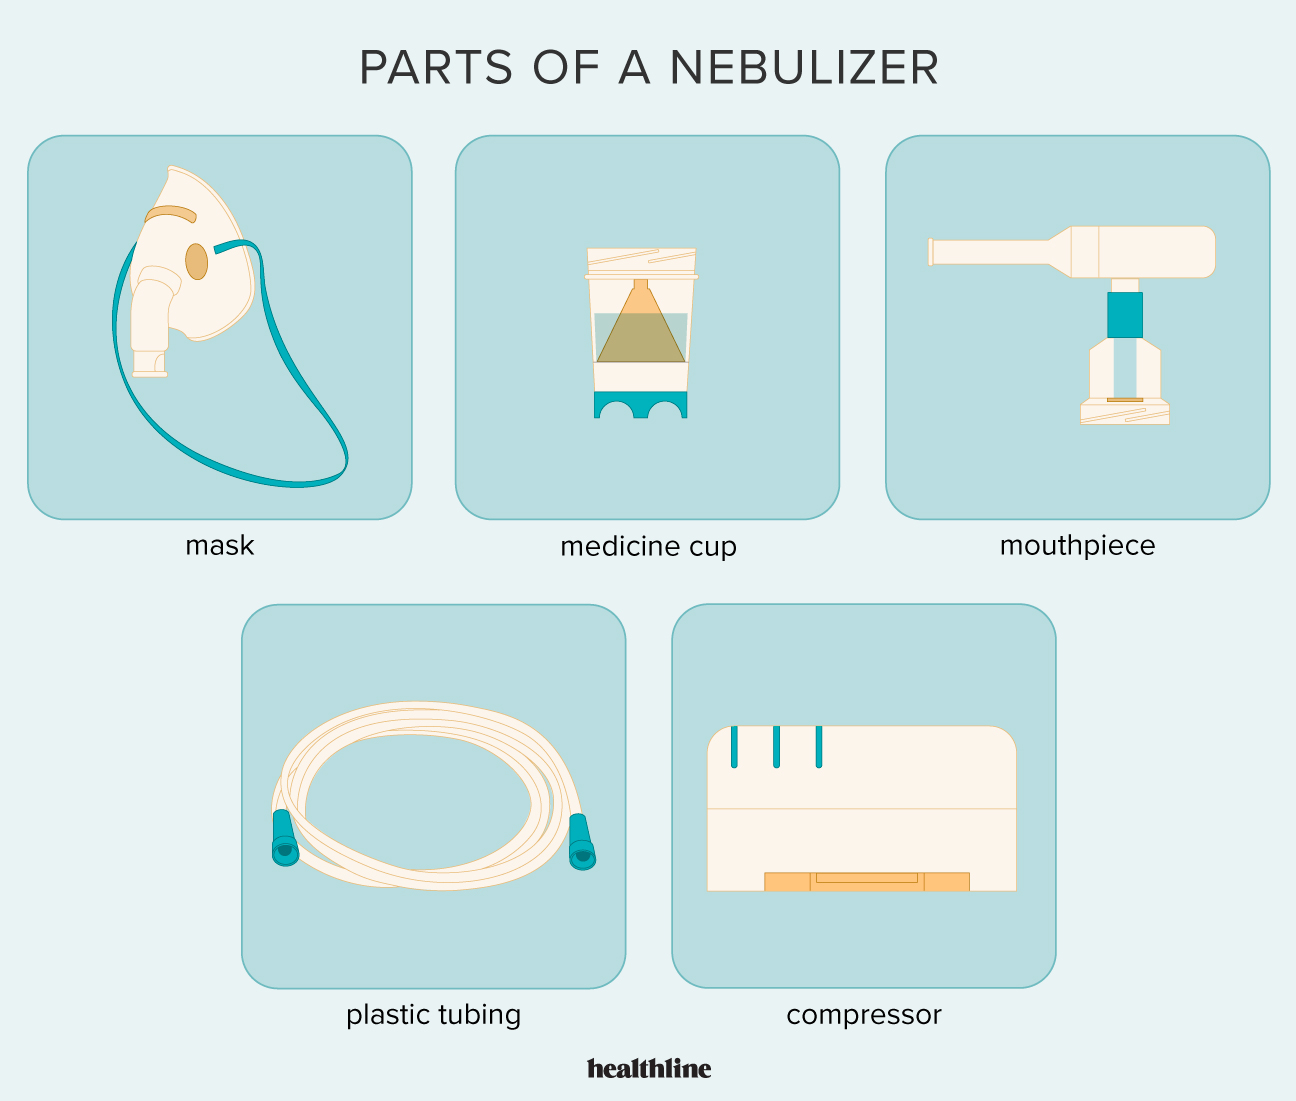
\includegraphics[scale=0.1]{type.jpg}
\caption{Parts of Nebulizers}
\end{figure}


%third paragraph
\subsection{Advantages}
Two advantages attributed to nebulizers are their ability to deliver larger dosages at a faster rate, especially in acute asthma; however, recent data suggests actual lung deposition rates are the same. In addition, another trial found that a MDI (with spacer) had a lower required dose for clinical result compared to a nebulizer.\\
Beyond use in chronic lung disease, nebulizers may also be used to treat acute issues like the inhalation of toxic substances. One such example is the treatment of inhalation of toxic hydrofluoric acid (HF) vapors. Calcium gluconate is a first-line treatment for HF exposure to the skin. By using a nebulizer, calcium gluconate is delivered to the lungs as an aerosol to counteract the toxicity of inhaled HF vapors.\\
The European Respiratory Society acknowledge that although nebulizers are used in hospitals and at home they suggest much of this use may not be evidence-based.



%last paragraph
\subsection{How it, works and is useful?}
A nebulizer delivers liquid medication via pressurized air. While individuals with asthma typically use both nebulizers and inhalers, occasionally, a  nebulizer may be easier to use — especially when it comes to young children who may not have the proper technique for an inhaler.\\
Examples of medications used in nebulizers include:\\
$Bronchodilators$ are drugs that help to open up the airway.
$Medical-grade saline (saltwater) solutions$ are solutions that help break up mucus in the lungs.\\
$Antibiotics$ are used to help treat or prevent infections.\\
Usually, the aerosolized medicine is inhaled through a tube-like mouthpiece, similar to that of an inhaler. The mouthpiece, however, is sometimes replaced with a face mask, similar to that used for inhaled anesthesia, for ease of use with young children or the elderly. Pediatric masks are often shaped like animals such as fish, dogs or dragons to make children less resistant to nebulizer treatments. Many nebulizer manufacturers also offer pacifier attachments for infants and toddlers. But mouthpieces are preferable if patients are able to use them since face-masks result in reduced lung delivery because of aerosol losses in the nose.

\subsection{Problems faced by person after using Nebulizer}

After use with corticosteroid, it is theoretically possible for patients to develop a yeast infection in the mouth (thrush) or hoarseness of voice (dysphonia), although these conditions are clinically very rare. To avoid these adverse effects, some clinicians suggest that the person who used the nebulizer should rinse his or her mouth. This is not true for bronchodilators; however, patients may still wish to rinse their mouths due to the unpleasant taste of some bronchodilating drugs, and one another thing we can consider.\\
 However, when airways become narrow — like during an asthma attack — an inhaler is most likely the best choice, because a nebulizer can take some time to set up.\\
\clearpage


\section{X-Ray Machine}


  It is a important medical devices use for imange purpose. which X-rays were first discovered on November 8, 1895,by the German physicist Wilhelm Conrad Röntgen. These first generation cold cathode or Crookes X-ray tubes were used until the 1920s. The Crookes tube was improved by William Coolidge in 1913.\\
  An X-ray is a common imaging test that’s been used for decades. It can help your doctor view the inside of your body without having to make an incision. This can help them diagnose, monitor, and treat many medical conditions.
Different types of X-rays are used for different purposes. For example, your doctor may order a mammogram to examine your breasts. Or they may order an X-ray with a barium enema to get a closer look at your gastrointestinal tract.\\
\begin{figure}[h]
\centering
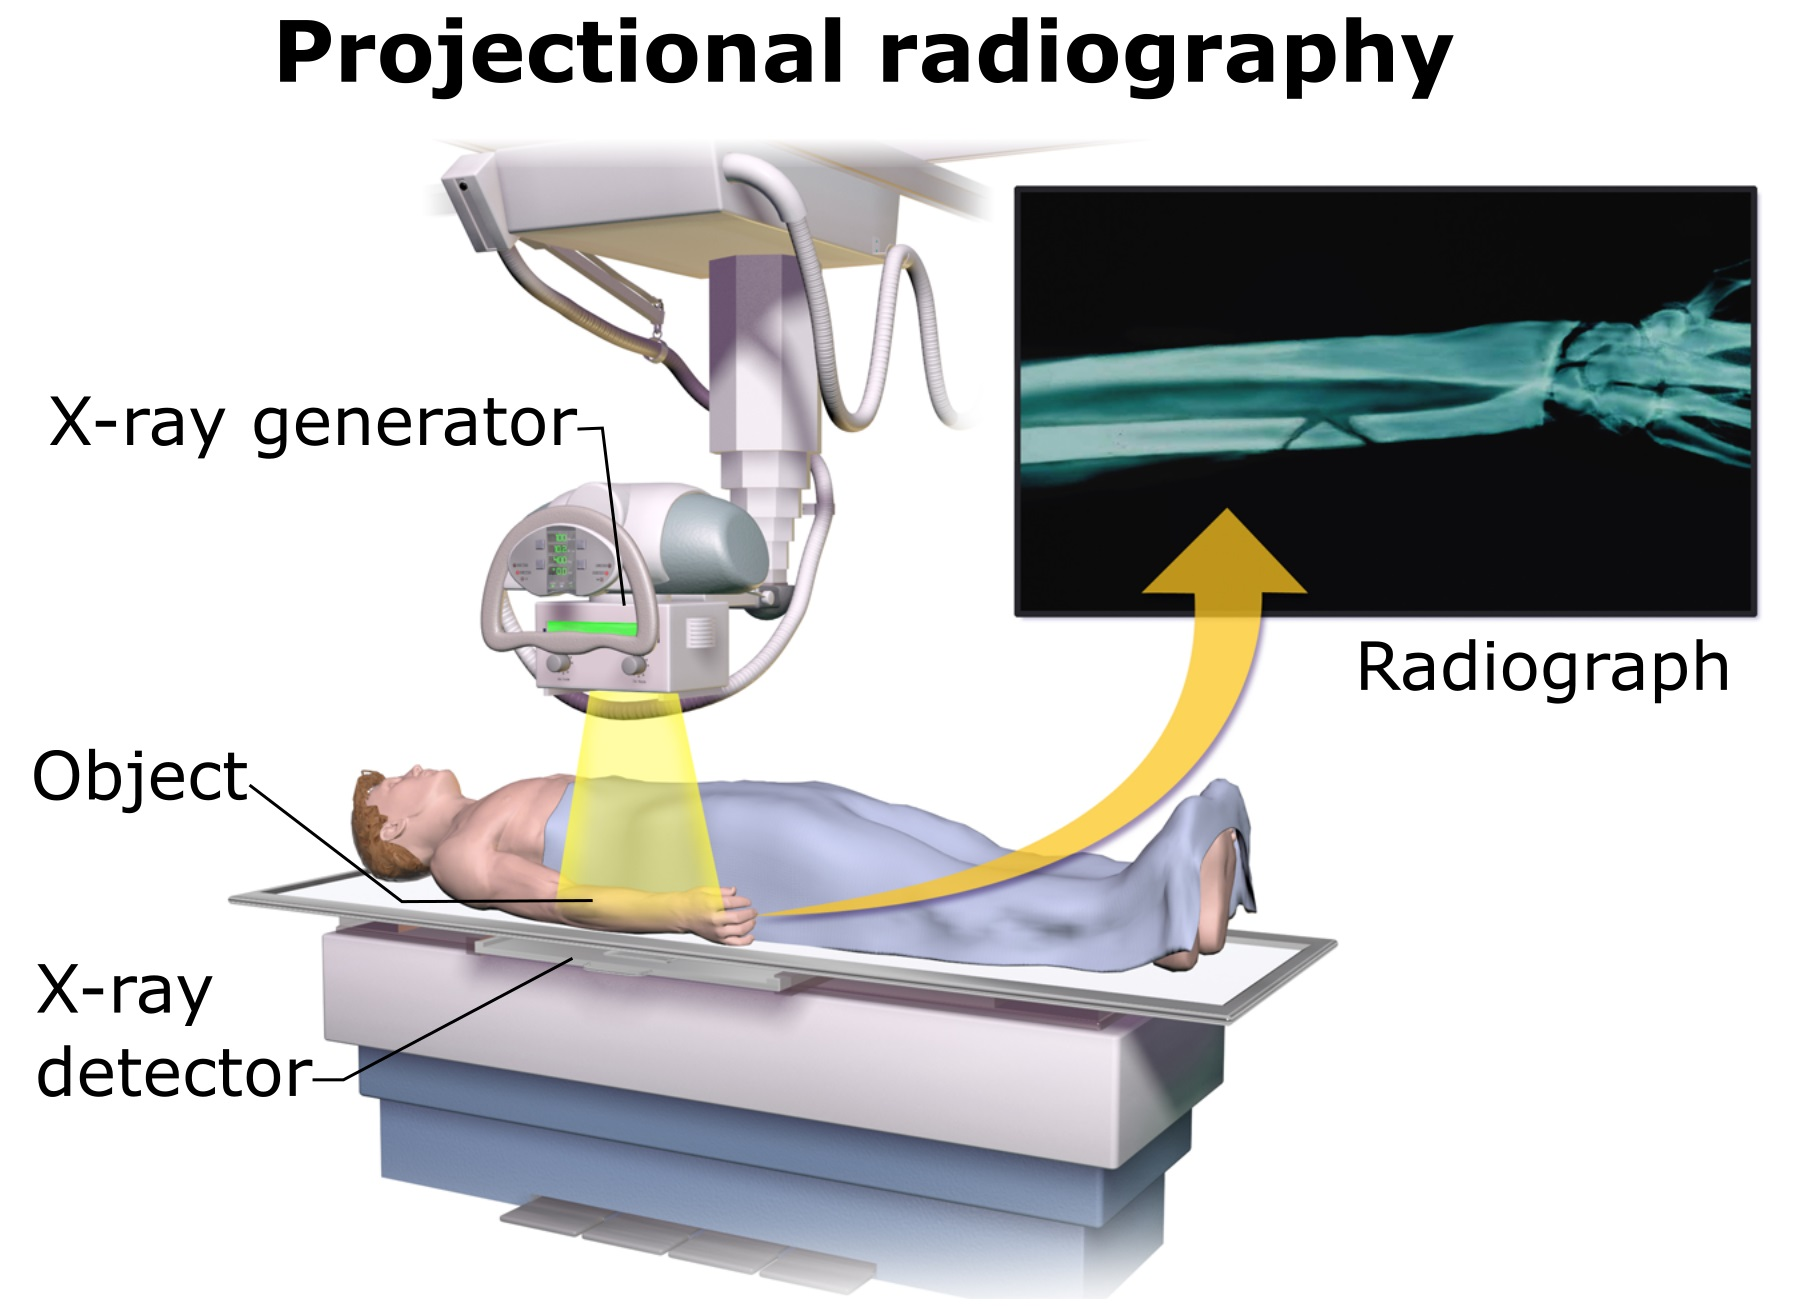
\includegraphics[scale=0.1]{xray.jpg}
\caption{X-Ray image}
\end{figure}
\subsection{Working principle}
To create a radiograph, a patient is positioned so that the part of the body being imaged is located between an x-ray source and an x-ray detector. When the machine is turned on, x-rays travel through the body and are absorbed in different amounts by different tissues, depending on the radiological density of the tissues they pass through. Radiological density is determined by both the density and the atomic number (the number of protons in an atom’s nucleus) of the materials being imaged.
\subsection{Used For}
X-ray radiography: Detects bone fractures, certain tumors and other abnormal masses, pneumonia, some types of injuries, calcifications, foreign objects, dental problems, etc.
\subsection{Risks}
X-rays use small amounts of radiation to create images of your body. The level of radiation exposure is considered safe for most adults, but not for a developing baby. If you’re pregnant or believe you could be pregnant, tell your doctor before you have an X-ray. They may suggest a different imaging method, such as an MRI.

If you’re having an X-ray done to help diagnose or manage a painful condition, such as a broken bone, you may experience pain or discomfort during the test. You will need to hold your body in certain positions while the images are being taken. This may cause you pain or discomfort. Your doctor may recommend taking pain medicine beforehand.

If you ingest a contrast material before your X-ray, it may cause side effects. These include:
\begin{itemize}
\item hives
\item itching
\item nausea
\item lightheadedness
\item a metallic taste in your mouth
\end{itemize}

In very rare cases, the dye can cause a severe reaction, such as anaphylactic shock, very low blood pressure, or cardiac arrest. In case of severe problem i would recommend to contact doctor immediately.
\subsection{Need Of improvement/Research}
\begin{itemize}
\item Greater mobility and portability
\item Better speed
\item Safer operation
\item Cost effective
\end{itemize}
\clearpage

\section{Hearing Aid}

A hearing aid is a device designed to improve hearing by making sound audible to a person with hearing loss. Hearing aids are classified as medical devices in most countries, and regulated by the respective regulations.\\ 
Modern devices are computerised electroacoustic systems that transform environmental sound to make it audible, according to audiometrical and cognitive rules.\\ 
Modern devices also utilize sophisticated digital signal processing to try and improve speech intelligibility and comfort for the user. Such signal processing includes feedback management, wide dynamic range compression, directionality, frequency lowering, and noise reduction.

Modern hearing aids require configuration to match the hearing loss, physical features, and lifestyle of the wearer. The hearing aid is fitted to the most recent audiogram and is programmed by frequency. This process is called "fitting" and is performed by a Doctor of Audiology, also called an audiologist (AuD), or by a Hearing Instrument Specialist (HIS). The amount of benefit a hearing aid delivers depends in large part on the quality of its fitting. Almost all hearing aids in use in the US are digital hearing aids.
\textbf{Devices similar to hearing aids include the osseointegrated auditory prosthesis (formerly called the bone-anchored hearing aid) and cochlear implant.}
\begin{figure}[h]
\centering
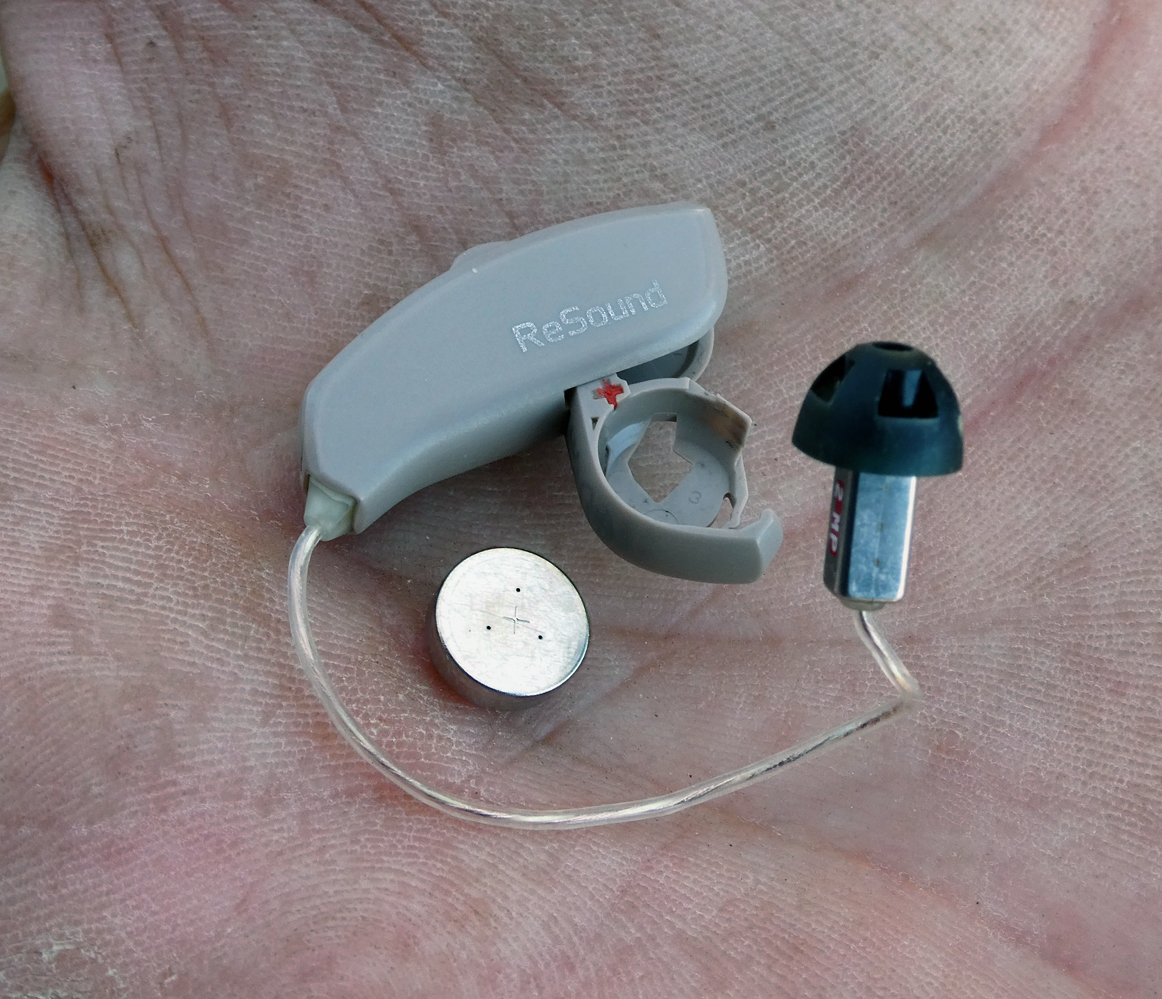
\includegraphics[scale=0.3]{hear.jpg}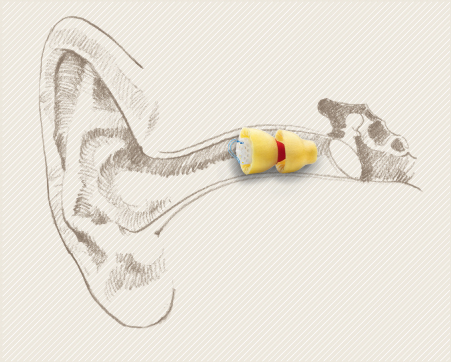
\includegraphics[scale=0.6]{hear1.jpg}
\caption{Hearing Aid images}
\end{figure}
\subsection{History}
The first hearing aids were ear trumpets, and were created in the 17th century. Some of the first hearing aids were external hearing aids. External hearing aids directed sounds in front of the ear and blocked all other noises. The apparatus would fit behind or in the ear.

The movement toward modern hearing aids began with the creation of the telephone, and the first electric hearing aid, the "akouphone", was created about 1895 by Miller Reese Hutchison. By the late 20th century, digital hearing aids were commercially available.\\
\subsection{Uses and Benefits}
Hearing aids are used for a variety of pathologies including sensorineural hearing loss, conductive hearing loss, and single-sided deafness. Hearing aid candidacy is typically determined by a Doctor of Audiology, or a certified hearing specialist, who will also fit the device based on the nature and degree of the hearing loss being treated. The amount of benefit experienced by the user of the hearing aid is multi-factorial, depending on the type, severity, and etiology of the hearing loss, the technology and fitting of the device, and on the motivation, personality, lifestyle, and overall health of the user.
Hearing aids are incapable of truly correcting a hearing loss; they are an aid to make sounds more audible. The most common form of hearing loss for which hearing aids are sought is sensorineural, resulting from damage to the hair cells and synapses of the cochlea and auditory nerve. $Sensorineural hearing loss$ reduces the sensitivity to sound, which a hearing aid can partially accommodate by making sound louder. Other decrements in auditory perception caused by sensorineural hearing loss, such as abnormal spectral and temporal processing, and which may negatively affect speech perception, are more difficult to compensate for using digital signal processing and in some cases may be exacerbated by the use of amplification.
$Conductive hearing losses$, which do not involve damage to the cochlea, tend to be better treated by hearing aids; the hearing aid is able to sufficiently amplify sound to account for the attenuation caused by the conductive component. Once the sound is able to reach the cochlea at normal or near-normal levels, the cochlea and auditory nerve are able to transmit signals to the brain normally.
\subsection{Types}
\begin{itemize}
\item Body worn
\item Behind the ear
\item In the ear
\item Invisible-ear-canal hearing Aid
\item CROS hearing aid
\end{itemize}

\subsection{How it can be more efficient?}
One approach is audiometry which measures a subject's hearing levels in laboratory conditions. The threshold of audibility for various sounds and intensities is measured in a variety of conditions. Although audiometric tests may attempt to mimic real-world conditions, the patient's own every day experiences may differ. An alternative approach is self-report assessment, where the patient reports their experience with the hearing aid.

Hearing aid outcome can be represented by three dimensions.
\begin{itemize}


\item hearing aid usage
\item aided speech recognition
\item benefit/satisfaction
\end{itemize}

The most reliable method for assessing the correct adjustment of a hearing aid is through real ear measurement. Real ear measurements (or probe microphone measurements) are an assessment of the characteristics of hearing aid amplification near the ear drum using a silicone probe tube microphone.

Current research is also pointing towards hearing aids and proper amplification as a treatment for tinnitus, a medical condition which manifests itself as a ringing or buzzing in the ears.
\clearpage


\section{Infusion Pump}
An infusion pump infuses fluids, medication or nutrients into a patient's circulatory system. It is generally used intravenously, although subcutaneous, arterial and epidural infusions are occasionally used.

Infusion pumps can administer fluids in ways that would be impractically expensive or unreliable if performed manually by nursing staff. For example, they can administer as little as 0.1 mL per hour injections (too small for a drip), injections every minute, injections with repeated boluses requested by the patient, up to maximum number per hour (e.g. in patient-controlled analgesia), or fluids whose volumes vary by the time of day.

Because they can also produce quite high but controlled pressures, they can inject controlled amounts of fluids subcutaneously (beneath the skin), or epidurally (just within the surface of the central nervous system – a very popular local spinal anesthesia for childbirth).


\begin{figure}[h]
\centering
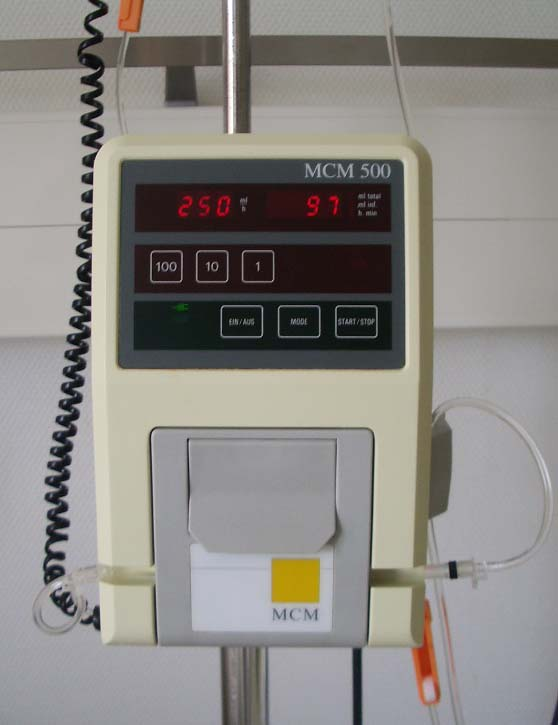
\includegraphics[scale=0.3]{infu.jpg}
\caption{Infusion pump image}
\end{figure}

\subsection{Types of infusion}

The user interface of pumps usually requests details on the type of infusion from the technician or nurse that sets them up:\\

Continuous infusion usually consists of small pulses of infusion, usually between 500 nanoliters and 10 milliliters, depending on the pump's design, with the rate of these pulses depending on the programmed infusion speed.
Intermittent infusion has a "high" infusion rate, alternating with a low programmable infusion rate to keep the cannula open. The timings are programmable. This mode is often used to administer antibiotics, or other drugs that can irritate a blood vessel.\\

To get the entire dose of antibiotics into the patient, the "volume to be infused" or VTBI must be programmed for at least 30 CCs more than is in the medication bag; failure to do so can potentially result in up to half of the antibiotic being left in the IV tubing.




\subsection{Types of pumps}

There are two basic classes of pumps:
\begin{enumerate}


\item Large volume pumps can pump fluid replacement such as saline solution, medications such as antibiotics or nutrient solutions large enough to feed a patient.
\item  Small-volume pumps infuse hormones, such as insulin, or other medicines, such as opiates.\\\\

Within these classes, some pumps are designed to be portable, others are designed to be used in a hospital, and there are special systems for charity and battlefield use


\end{enumerate}

























\clearpage

\section{Stretcher}
An early stretcher, likely made of wicker over a frame, appears in a manuscript from c.1380. Simple stretchers were common with militaries right through the middle of the 20th century.\\

A stretcher, or litter is an apparatus used for moving patients who require medical care. A basic type (cot or litter) must be carried by two or more people. A wheeled stretcher (known as a gurney, trolley, bed or cart) is often equipped with variable height frames, wheels, tracks, or skids. Stretchers are primarily used in acute out-of-hospital care situations by emergency medical services (EMS), military, and search and rescue personnel. In medical forensics the right arm of a corpse is left hanging off the stretcher to let paramedics know it is not a wounded patient.
\begin{figure}[h]
\centering
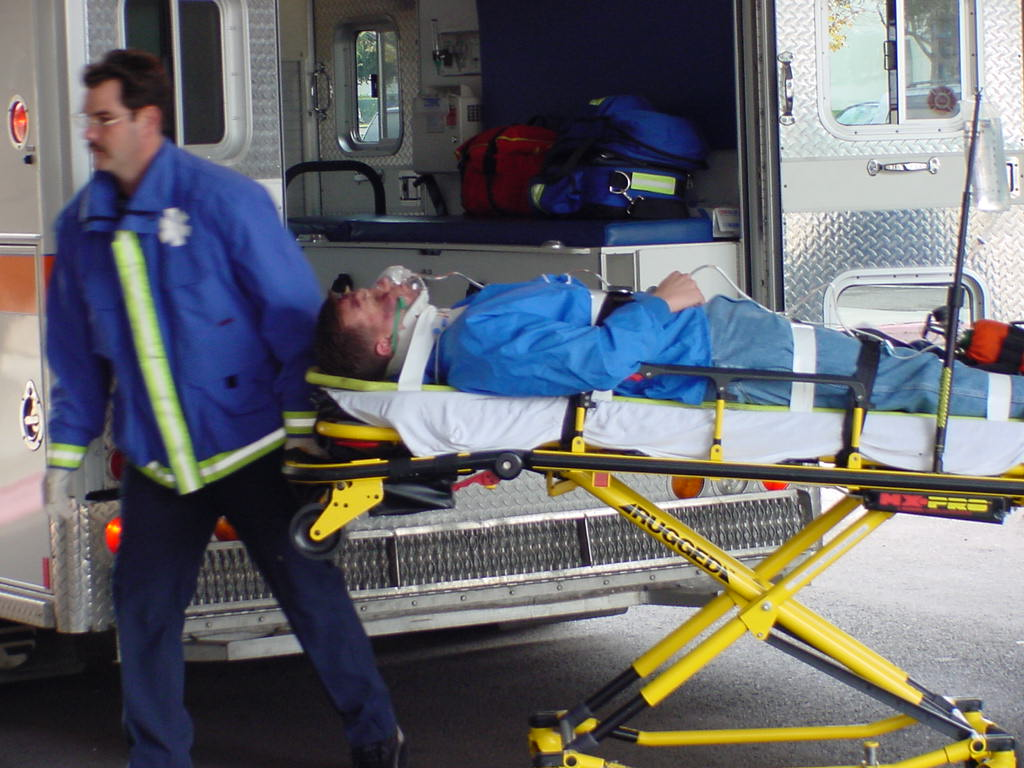
\includegraphics[scale=0.3]{stre.jpg}
\caption{stretcher image}
\end{figure}

\subsection{Basic stretchers}
\begin{itemize}


\item Simple stretchers are the most rudimentary type. They are lightweight and portable, made of canvas or other synthetic material suspended between two poles or tubular aluminum frame. Many are stored as disaster supplies and are often former military equipment.
\begin{figure}[h]
\centering
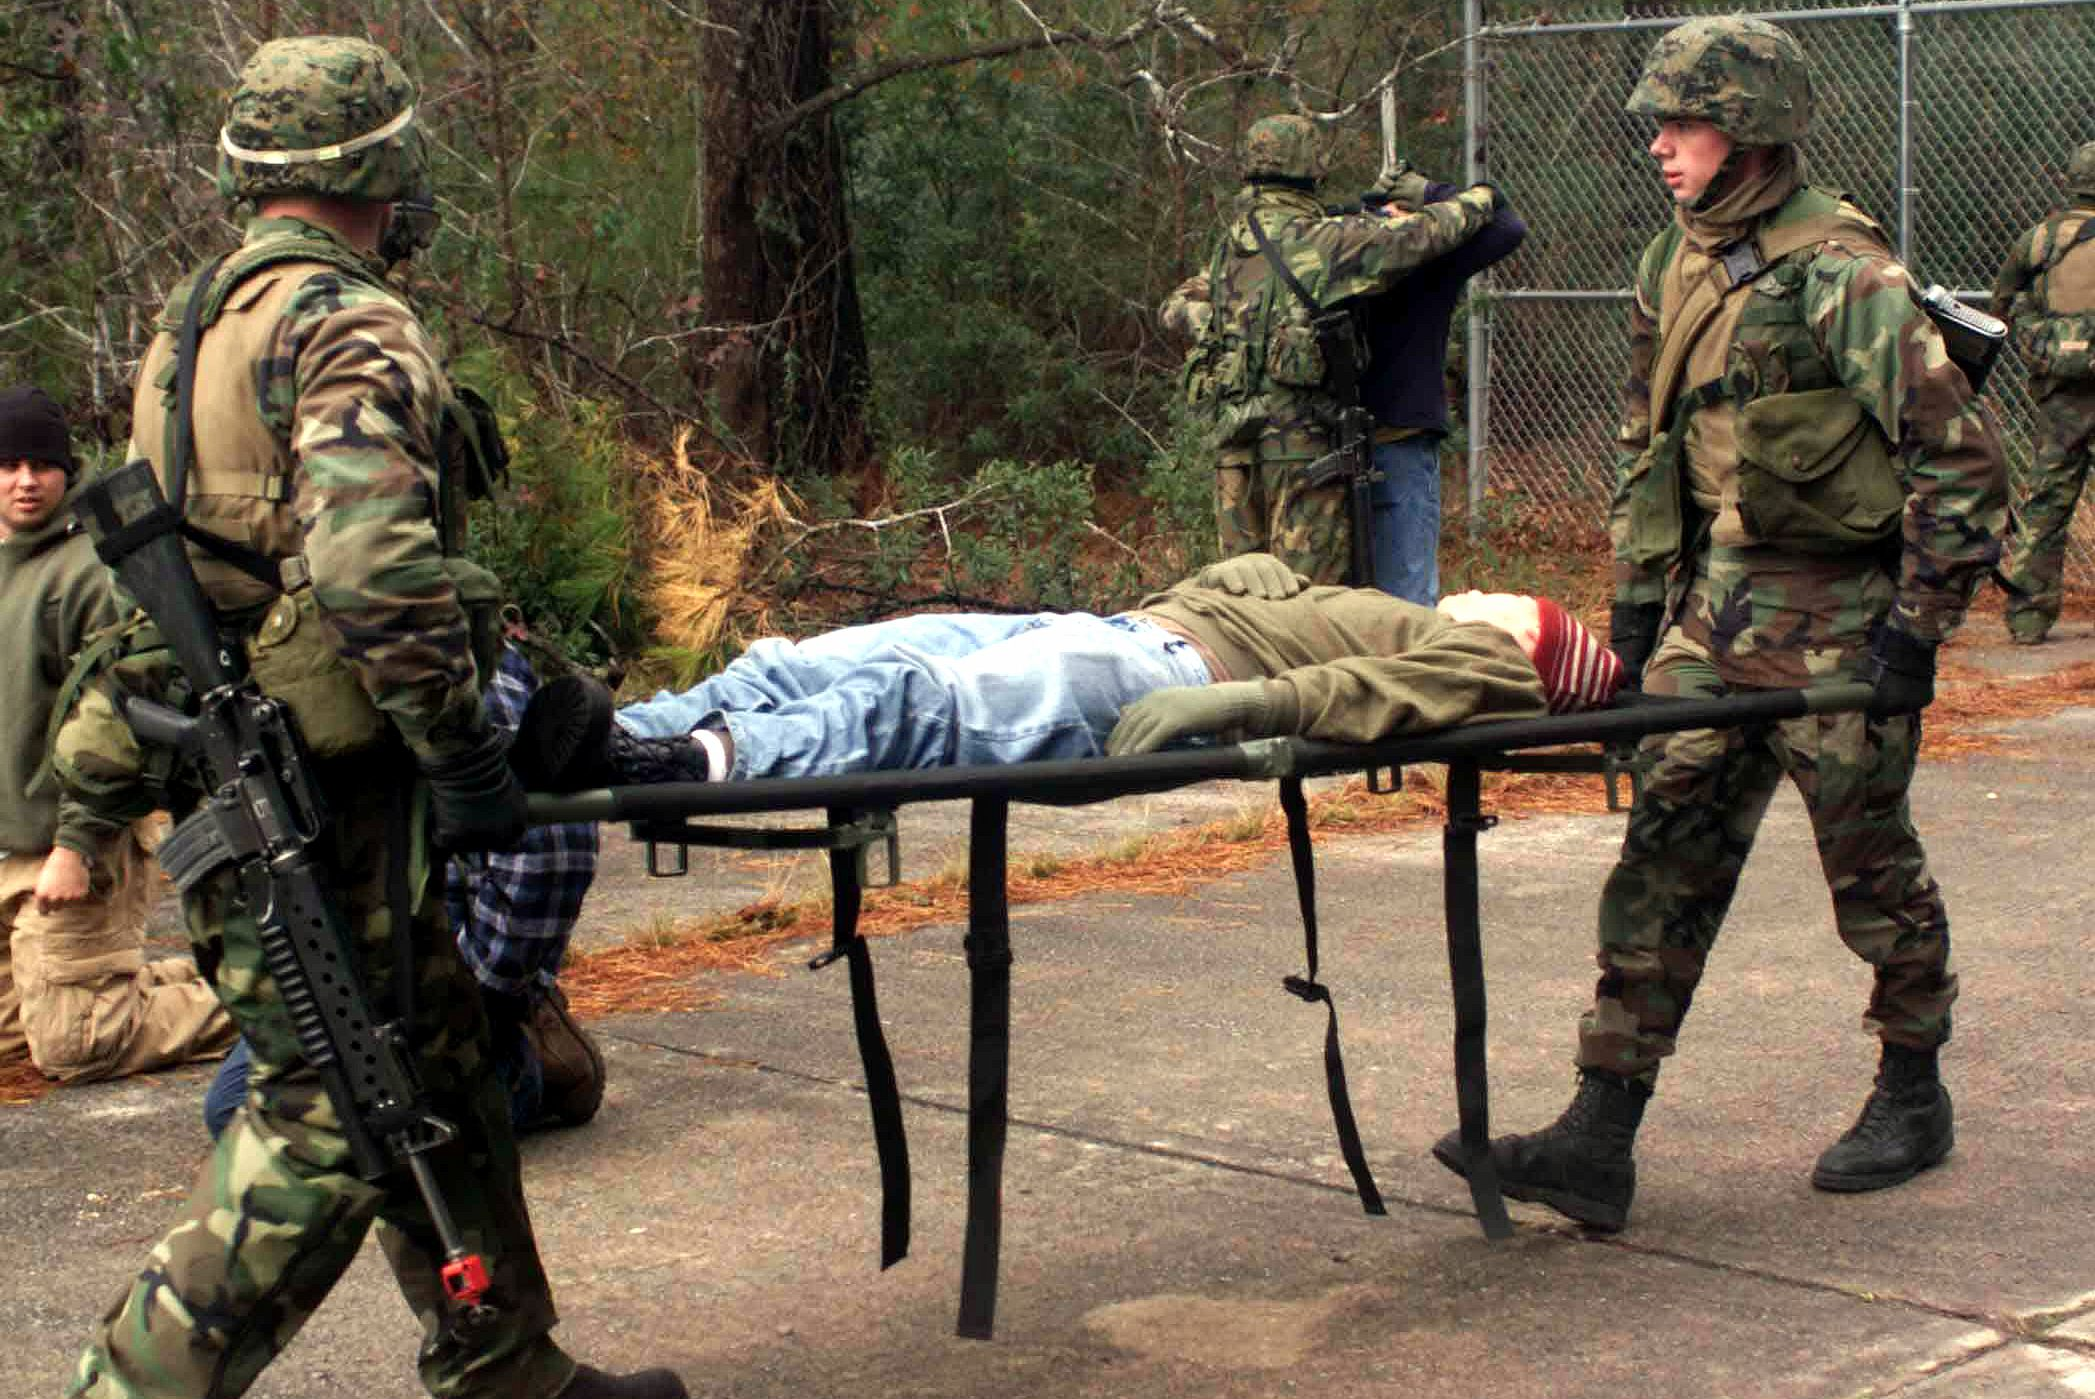
\includegraphics[scale=0.1]{str.jpg}
\caption{stretcher image}
\end{figure}

\item The WauK board is also designed for use in small spaces. The patient is secured to the board with straps. It has two wheels and a foldable footrest at one end, allowing the patient to be moved by one person, much as with a hand truck for moving cargo. It can also be used at a variety of angles, making it easier to traverse obstacles, such as tight stairwells.\\

\subsection{Wheeled stretchers} 
For ambulances, a collapsible wheeled stretcher, or gurney, is a type of stretcher on a variable-height wheeled frame. Normally, an integral lug on the stretcher locks into a sprung latch within the ambulance in order to prevent movement during transport, often referred to as antlers due to their shape. It is usually covered with a disposable sheet and cleaned after each patient in order to prevent the spread of infection. Its key value is to facilitate moving the patient and sheet onto a fixed bed or table on arrival at the emergency department. Both types may have straps to secure the patient

\end{itemize}




\textbf{This assignment is made under the supervision of
\emph{Dr.Saurav Gupta Sir.}}

\end{document}
